% !TEX root =  ../../thesis.tex
\section{Appearance Representation and Model}\label{sec:notation:appearance}
As explained in Sec.~\ref{sec:deformable_models_review}, Deformable Models can
be split in two categories based on whether they utilize
\emph{(i)}~\emph{holistic} or \emph{(ii)}~\emph{part-based} appearance
representation. Figure~\ref{fig:holistic_partbased_example} shows such an
example. Additionally, all Deformable Models employ a feature-based image
representation.

\subsection{Feature Extraction}
Features are computed by applying a \emph{feature extraction function} that
attempts to describe distinctive and important image characteristics (\eg,
SIFT~\cite{lowe1999object}, HOG~\cite{dalal2005histograms}). Given an
input image $\mathbf{I}$ with size $H\times W$, the feature extraction function
$\mathcal{F}(\mathbf{I})$ is defined as
%%%%%%%%%%%%%%%%
\begin{equation}
  \mathcal{F}:\mathbb{R}^{H\times W} \longrightarrow \mathbb{R}^{H'\times W'\times D}
\end{equation}
%%%%%%%%%%%%%%%%
where $H'\times W'$ is the size of the output feature-based image and $D$ is
the number of channels. Note that feature functions can be separated in two
categories: \emph{(i)}~\emph{densely-sampled} and
\emph{(ii)}~\emph{sparsely-sampled}. Densely-sampled features extract a feature
vector per image pixel, thus $H'=H$ and $W'=W$. On the other hand,
sparsely-sampled features extract feature vectors from downsampled image
locations, thus $H'<H$ and $W'<W$.

By denoting the input image in vectorial form $\mathbf{t}$ with size
$HW\times 1$, the feature extraction function is redefined as
%%%%%%%%%%%%%%%%
\begin{equation}
  \mathcal{F}: \mathbb{R}^{HW} \longrightarrow \mathbb{R}^m
  \label{equ:feature_function}
\end{equation}
%%%%%%%%%%%%%%%%
which returns a feature-vector of length $m=H'W'D$.

\subsection{Holistic Appearance Representation}\label{sec:notation_holistic}
A holistic appearance representation aims to warp all the texture information
within a shape instance to a reference shape (canonical space). In general, a
warp function maps the points within a source shape to their corresponding
coordinates in a target shape. In the Deformable Models literature, the warp
function is commonly referred to as \emph{motion model} and denoted as
$\mathcal{W}(\mathbf{p})$. Its role is to extrapolate the position of all the
pixels inside the convex hull of the reference shape to a particular shape
instance $\mathbf{s}$ (generated using the shape parameters $\mathbf{p}$ as
shown in Eq.~\ref{equ:shape_generation}) based on their relative position with
respect to the sparse landmarks (for which direct correspondences are always
known).

As also discussed and proved in Chapter~\ref{ch:aam}, it is more beneficial to
warp the extracted features rather than extracting features on the warped
image. Thus, given an input image $\mathbf{I}$ with size $H\times W$ and its
vectorized form $\mathbf{t}$, we can define a holistic feature-based appearance vector as
%%%%%%%%%%%%%%
\begin{equation}
  \mathbf{f} = \mathbf{t}_{\mathcal{F}}\left(\mathcal{W}(\mathbf{p})\right) \text{ with } \mathbf{t}_{\mathcal{F}} = \mathcal{F}(\mathbf{t})
  \label{equ:holistic_appearance}
\end{equation}
%%%%%%%%%%%%%%
where the feature extraction is based on Eq.~\ref{equ:feature_function}.

In this thesis, we employ the Piecewise Affine Warp
(PWA)~\cite{cootes2004statistical,matthews2004active}, which performs the
mapping based on the barycentric coordinates of the corresponding triangles
between the two shapes that are extracted using Delaunay
Triangulation~\cite{lee1980two}. An example of such an appearance
representation is shown in Fig.~\ref{fig:holistic}. Other warping methods could
also be employed, such as Thin Plate Splines
(TPS)~\cite{cootes2004statistical,papandreou2008adaptive}.

%%%%%%%%%%%%%%
\begin{figure}[!t]
\centering
%%%%%%%%%
\subfloat[Original image annotated with a set of $n$ sparse landmarks.]{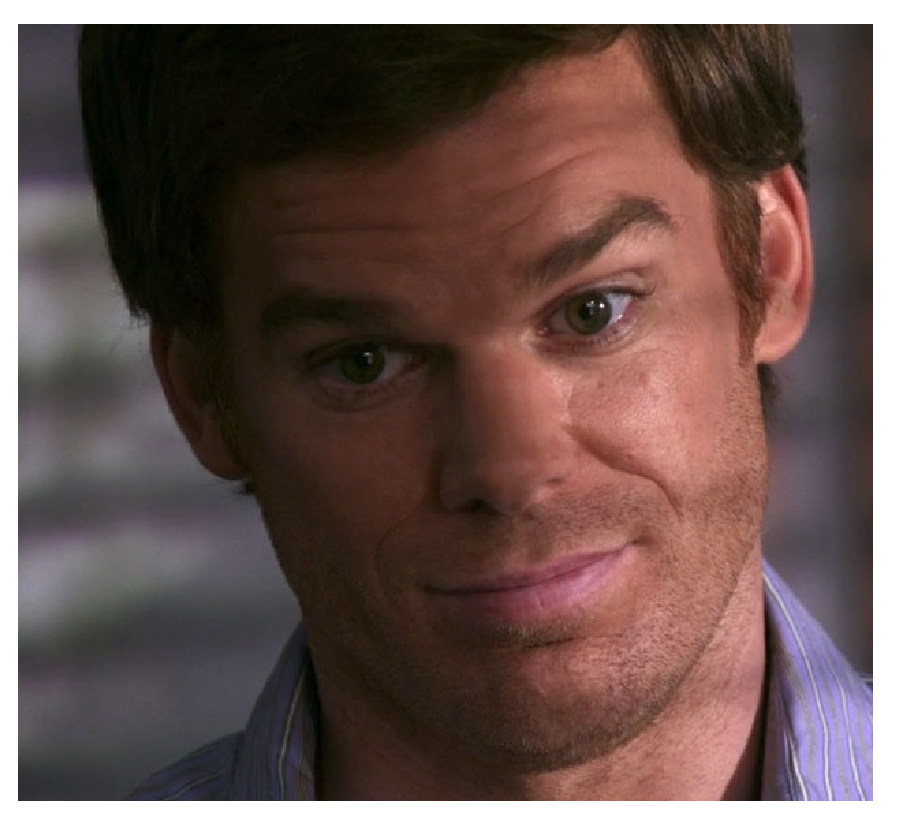
\includegraphics[width=0.3\linewidth]{figures/notation/holistic_partbased/original}}
\hfill
\subfloat[Holistic appearance representation using Piecewise Affine Warp.]{\includegraphics[width=0.3\linewidth]{figures/notation/holistic_partbased/holistic}\label{fig:holistic}}
\hfill
\subfloat[Part-based appearance representation by extracting patches centered around the landmarks.]{\includegraphics[width=0.3\linewidth]{figures/notation/holistic_partbased/part_based}}
%%%%%%%%%
\caption{Example of holistic and part-based appearance representation based on a sparse shape.}
\label{fig:holistic_partbased_example}
\end{figure}
%%%%%%%%%%%%%%

\subsection{Part-Based Appearance Representation}\label{sec:notation:part_based}
The scientific community has lately turned towards part-based appearance
representation, \ie, extracting appearance patches centered around the landmark
coordinates. Although this depends on the object class and application, in
general, the part-based representation has proved to be more efficient than the
holistic as the warp function is replaced by a simple sampling function and
it is also more natural for articulated rigid objects (\eg, body pose, hand,
etc.). Let us denote the vectorized form of an $h\times w$ image patch that
corresponds to the image location
$\boldsymbol{\ell}_i=\left[x_i, y_i\right]^{\mathsf{T}}$ as the $hw\times 1$
vector
%%%%%%%%%%%%%%
\begin{equation}
  \mathbf{t}_{\boldsymbol{\ell}_i} = \left[ \mathbf{I}(\mathbf{z}_1), \mathbf{I}(\mathbf{z}_2), \ldots, \mathbf{I}(\mathbf{z}_{hw}) \right]^{\mathsf{T}},~\left\lbrace \mathbf{z}_j \right\rbrace_{j=1}^{hw} \in \boldsymbol{\Omega}_{\boldsymbol{\ell}_i}
\end{equation}
%%%%%%%%%%%%%%
where $\mathbf{\Omega}_{\boldsymbol{\ell}_i}$ is a set of discrete neighboring
pixel locations $\mathbf{z}_j=[x_j,y_j]^{\mathsf{T}}$ within a rectangular
region centered at location $\boldsymbol{\ell}_i$ and $hw$ is the image patch
vector's length. By using the feature extraction function of
Eq.~\ref{equ:feature_function}, the procedure of extracting a feature-based
vector from a patch centered at a given image location can be denoted as
%%%%%%%%%%%%%%
\begin{equation}
  \mathcal{F}(\mathbf{t}_{\boldsymbol{\ell}_i}) \equiv \mathcal{F}\left(\left[\mathbf{I}(\mathbf{z}_1), \mathbf{I}(\mathbf{z}_2), \ldots, \mathbf{I}(\mathbf{z}_{hw})\right]^{\mathsf{T}}\right),~\left\lbrace \mathbf{z}_j \right\rbrace_{j=1}^{hw} \in \boldsymbol{\Omega}_{\boldsymbol{\ell}_i}
\end{equation}
%%%%%%%%%%%%%%
Consequently, given a shape instance of the form of Eq.~\ref{equ:shape}, the
corresponding \emph{part-based appearance vector} $\mathbf{f}$ is an
$mn\times 1$ vector that consists of the concatenation of the vectorized
feature-based image patches that correspond to the $n$ landmarks of the shape
instance, \ie
%%%%%%%%%%%%%%
\begin{equation}
  \mathbf{f}(\mathbf{s}) = \left[ \mathcal{F}(\mathbf{t}_{\boldsymbol{\ell}_1})^{\mathsf{T}}, \mathcal{F}(\mathbf{t}_{\boldsymbol{\ell}_2})^{\mathsf{T}}, \ldots,
  \mathcal{F}(\mathbf{t}_{\boldsymbol{\ell}_n})^{\mathsf{T}} \right]^{\mathsf{T}}
  \label{equ:part_based_appearance}
\end{equation}
%%%%%%%%%%%%%%
where $\mathbf{s}$ is given by Eq.~\ref{equ:shape}.

\subsection{Appearance Model}\label{sec:notation:appearance_model}
Given a set of $N$ appearance vector samples
$\left\lbrace \mathbf{f}_1, \ldots, \mathbf{f}_N\right\rbrace$
that are extracted using either Eq.~\ref{equ:holistic_appearance} or
Eq.~\ref{equ:part_based_appearance}, we can apply PCA to obtain a parametric
statistical linear appearance model. By keeping the first $n_a$ principal components, we end up with
%%%%%%%%%%%%%%
\begin{equation}
  \left\lbrace \mathbf{U}_a, \bar{\mathbf{a}} \right\rbrace
\end{equation}
%%%%%%%%%%%%%%
where $\mathbf{U}_a \in \mathbb{R}^{m\times n_a}$ is the orthonormal basis and
$\bar{\mathbf{a}} \in \mathbb{R}^{m}$ is the mean appearance vector. This
model can be used to generate new appearance instances using the function
$\mathcal{A}: \mathbb{R}^{n_a} \longrightarrow \mathbb{R}^m$ as
%%%%%%%%%%%%%%
\begin{equation}
  \mathbf{a}_{\mathbf{c}} = \mathcal{A}(\mathbf{c}) \equiv \bar{\mathbf{a}} + \mathbf{U}_a\mathbf{c}
  \label{equ:appearance_generation}
\end{equation}
%%%%%%%%%%%%%%
where
%%%%%%%%%%%%%%
\begin{equation}
\mathbf{c} = \left[ c_1, c_2, \ldots, c_{n_a} \right]^{\mathsf{T}}
\label{equ:appearance_parameters}
\end{equation}
%%%%%%%%%%%%%%
is the $n_a\times1$ vector of \emph{appearance parameters} that control the
linear combination of the eigenvectors.

Figures~\ref{fig:holistic_appearance_model_instances} and ~\ref{fig:part_based_appearance_model_instances} show some exemplar appearance
instances generated using the first five principal components of a holistic and
a part-based appearance model, respectively. Note that both models are trained
on grayscale intensities, in order to make the variance visualization more
comprehensive. The figures vary the parameter that corresponds to each component
using the values
$\left\lbrace -3\sqrt{\lambda_i}, -\frac{3}{2}\sqrt{\lambda_i}, \frac{3}{2}\sqrt{\lambda_i}, 3\sqrt{\lambda_i}\right\rbrace,~\forall i=1,\ldots,5$
where $\lambda_i$ denotes the corresponding eigenvalue.
